%%%%%%%%%%%%%%%%%%%%%%%%%%%%%%%%%%%%%%%%%
% Journal Article
% LaTeX Template
% Version 1.4 (15/5/16)
%
% This template has been downloaded from:
% http://www.LaTeXTemplates.com
%
% Original author:
% Frits Wenneker (http://www.howtotex.com) with extensive modifications by
% Vel (vel@LaTeXTemplates.com)
%
% License:
% CC BY-NC-SA 3.0 (http://creativecommons.org/licenses/by-nc-sa/3.0/)
%
%%%%%%%%%%%%%%%%%%%%%%%%%%%%%%%%%%%%%%%%%
%----------------------------------------------------------------------------------------
%	PACKAGES AND OTHER DOCUMENT CONFIGURATIONS
%----------------------------------------------------------------------------------------

\documentclass[twoside,twocolumn]{article}

\usepackage{blindtext} % Package to generate dummy text throughout this template

\usepackage[sc]{mathpazo} % Use the Palatino font
\usepackage[utf8]{inputenc}
\usepackage[T1]{fontenc} % Use 8-bit encoding that has 256 glyphs
\linespread{1.05} % Line spacing - Palatino needs more space between lines
\usepackage{microtype} % Slightly tweak font spacing for aesthetics

\usepackage[english]{babel} % Language hyphenation and typographical rules

\usepackage[hmarginratio=1:1,top=32mm,columnsep=20pt]{geometry} % Document margins
\usepackage[hang, small,labelfont=bf,up,textfont=it,up]{caption} % Custom captions under/above floats in tables or figures
\usepackage{booktabs} % Horizontal rules in tables

\usepackage{lettrine} % The lettrine is the first enlarged letter at the beginning of the text

\usepackage{enumitem} % Customized lists
\setlist[itemize]{noitemsep} % Make itemize lists more compact

\usepackage{abstract} % Allows abstract customization
\renewcommand{\abstractnamefont}{\normalfont\bfseries} % Set the "Abstract" text to bold
\renewcommand{\abstracttextfont}{\normalfont\small\itshape} % Set the abstract itself to small italic text

\usepackage{titlesec} % Allows customization of titles
\renewcommand\thesection{\Roman{section}} % Roman numerals for the sections
\renewcommand\thesubsection{\roman{subsection}} % roman numerals for subsections
\titleformat{\section}[block]{\large\scshape\centering}{\thesection.}{1em}{} % Change the look of the section titles
\titleformat{\subsection}[block]{\large}{\thesubsection.}{1em}{} % Change the look of the section titles

\usepackage{fancyhdr} % Headers and footers
\pagestyle{fancy} % All pages have headers and footers
\fancyhead{} % Blank out the default header
\fancyfoot{} % Blank out the default footer
\fancyhead[C]{Running title $\bullet$ May 2016} % Custom header text
\fancyfoot[RO,LE]{\thepage} % Custom footer text

\usepackage{titling} % Customizing the title section

\usepackage{hyperref} % For hyperlinks in the PDF

\usepackage{graphicx}

\usepackage{csquotes}
\usepackage[style=ieee,backend=bibtex]{biblatex}

\bibliography{biblio}

%----------------------------------------------------------------------------------------
%	TITLE SECTION
%----------------------------------------------------------------------------------------

\setlength{\droptitle}{-4\baselineskip} % Move the title up

\pretitle{\begin{center}\normalsize Comments on : \\
\Huge\bfseries} % Article title formatting
\posttitle{\end{center}} % Article title closing formatting
\title{\citetitle{pomerleau_review_2015}} % Article title
\author{%
\textsc{Virgile Daugé}\thanks{A thank you or further information} \\[1ex] % Your name
\normalsize University of Lorraine \\ % Your institution
\normalsize \href{mailto:virgile.dauge@inria.fr}{virgile.dauge@inria.fr} % Your email address
%\and % Uncomment if 2 authors are required, duplicate these 4 lines if more
%\textsc{Jane Smith}\thanks{Corresponding author} \\[1ex] % Second author's name
%\normalsize University of Utah \\ % Second author's institution
%\normalsize \href{mailto:jane@smith.com}{jane@smith.com} % Second author's email address
}
\date{\today} % Leave empty to omit a date
\renewcommand{\maketitlehookd}{%

%----------------------------------------------------------------------------------------
%	Abstract
%----------------------------------------------------------------------------------------

\begin{abstract}
\noindent The scope of this work is to present registration algorithms and their
use in mobile robotics.
\end{abstract}
}

%----------------------------------------------------------------------------------------

\begin{document}

% Print the title
\maketitle

%----------------------------------------------------------------------------------------
%	ARTICLE CONTENTS
%----------------------------------------------------------------------------------------

\section{Introduction}

\lettrine[nindent=0em,lines=3]{R}egistration algorithms associate sets of data
into a common coordinate system by minimizing the alignment error.

PB : Unless two identical shapes are registered
together, outliers that are not present in both shapes need to be iden-
tified.

primitives derived from points are too sensitive to
noise and are not stable in moving systems with current (1994) sens-
ing capabilities.
=> points were more reliable

need to handle dynamic elements.

difficulty to find a single versatile ICP version.

The aim of geometric registration is to be able to represent a shape,
called reading, in the same coordinate frame as another, called
reference.
This is equivalent to finding the transformation of reading
that best aligns it to reference.

\begin{figure}
  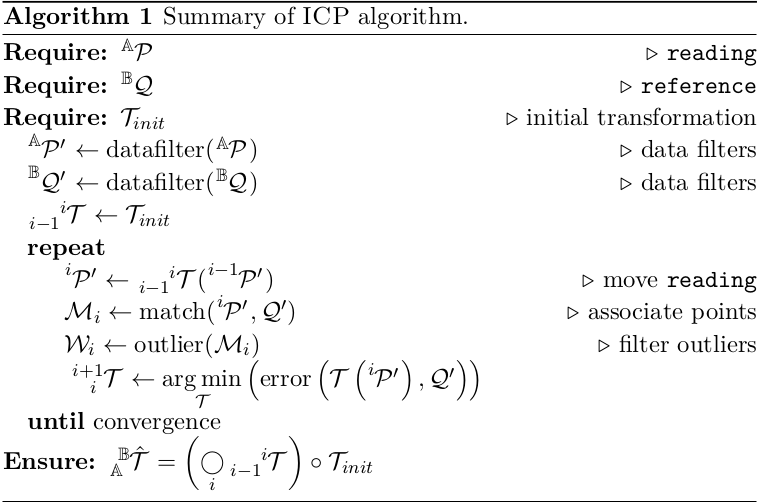
\includegraphics[angle=90,width=7cm]{ICPalgo}
  \caption{ICP algorithm}
  \label{fig:ICPalgo}
\end{figure}

\subsection{sensors}
\subsubsection{laser rangefinders (lidars)}
\subsubsection{cameras}
Light field capture simultaneously multiple focus
points and reconstruct images with different depth of fields out of the
recorded data.


\subsection{transformations}
\begin{description}
  \item[Rigid transformation] is a combination of translation and rotation.
It is also known as a Euclidean transformation.
\item[Similarity transform] is a combination of rigid transformation and
uniform scaling.
\item[Affine transform] is a combination of rigid transformation, nonuni-
form scaling and shear.
\item[Orthogonal projection] is a group of transformation based on vector
and planar projection.
\end{description}

The initial transformation is a sensitive part of registration al-
gorithms when the data association is realized mainly based on geo-
metric features.

\subsection{feature enhancement}
most of the shapes encountered in the a real environ-
ment are too complex to be completely synthesized with parameters

fives types of primitives :
\begin{itemize}
  \item point,
  \item line,
  \item plane,
  \item curve and
  \item quadric
\end{itemize}


The ratio of noise to signal is often higher in
robotics than in object modeling, thus rendering many complex mod-
eling algorithms ineffective. This could explain why most registration
algorithms applied to robotics tend to select a shape representation
very close to the raw measurements (i.e., points) instead of relying on
faulty surface reconstruction.

\subsection{Descriptor enhancement}

using the intensity remission
combined with cameras to add color information
techniques are used to reduce the number of features: random sampling, grid projection, octree and bounding box.

\subsection{data association}
In laser rangefinder based
matching, feature positions are quite accurate compared to descrip-
tor uniqueness but the initial transformation needs to be within
a maximum range to avoid local minima

When using descriptors, the
matching becomes independent of the initial position, but may fail for
repetitive elements

kD-tree is better in terms of accuracy, query time, build time,
and memory usage
%------------------------------------------------

\section{Methods}
\blindtext


%------------------------------------------------

\section{Results}
\blindtext

%------------------------------------------------

\section{Discussion}
\subsection{Current state}
\blindtext
\subsection{Possibles enhancements}
\blindtext

\printbibliography
\end{document}
